\documentclass{report}
\usepackage[top=3.5cm, bottom=4cm, left=3.1cm, right=3.1cm, headsep=14pt]{geometry}
\usepackage{amsmath}

\usepackage[english]{babel}
\usepackage[utf8x]{inputenc}
\usepackage{amsmath}
\usepackage{graphicx}
\usepackage{subfig}
\usepackage{pdfpages}
\usepackage{tex/algorithm2e}
\usepackage{tex/algorithmic}
\usepackage{float}
\usepackage{hyperref}
\usepackage{fancyhdr}
\pagestyle{fancy}
%fancyhead[LE,RO]{}
%fancyhead[LO,RE]{\slshape \leftmark}
\fancyhead[RE]{\rightmark}
\fancyhead[LE,RO]{}
%\fancyhead[LO,RE]{}
%\bibliographystyle{plos2009}
\bibliographystyle{apalike}

\cfoot{\thepage}

\DeclareMathAlphabet      {\mathbfit}{OML}{cmm}{b}{it}

\def\s{\sigma}
\newcommand{\slfrac}[2]{\left.#1\middle/#2\right.}

% New definition of square root:
% it renames \sqrt as \oldsqrt
\let\oldsqrt\sqrt
% it defines the new \sqrt in terms of the old one
\def\sqrt{\mathpalette\DHLhksqrt}
\def\DHLhksqrt#1#2{%
    \setbox0=\hbox{$#1\oldsqrt{#2\,}$}\dimen0=\ht0
    \advance\dimen0-0.2\ht0
    \setbox2=\hbox{\vrule height\ht0 depth -\dimen0}%
{\box0\lower0.4pt\box2}}



\begin{document}
\chapter*{Acknowledgement}
%\section*{Acknowledgement}
\addcontentsline{toc}{chapter}{Acknowledgements}

This thesis represents the work I have carried out as a PhD student under the supervision of Professor Jan H. Jensen in his group of Biocomputational Chemistry.
Thank you to all who have supported me during my work at the third floor of C-building at the H.C. Ørsteds Institute.
\\\\I would especially like to thank the following people:

\begin{itemize}
\item Thank you to my supervisor, Jan "Yoda" Jensen for introducing me to the
    exciting fields of quantum chemistry and biocomputational chemistry, teaching me everything I know (and more), for your patience, and the inspiration you bring to everyone around you.

\item Thank you to Jens Breinholt at Novo Nordisk for supporting me with my work -- I sincerely hope, that my work will very soon become practically useable. And thank you to the Novo Nordisk STAR PhD program for financial support, and for giving me the opportunity to carry out this study.

\item Thank you to all of our collaborators at the Biocenter, who always have been very supportive. Especially, Thomas Hamelryck (in the presence of whom everything is trivially solved using Bayes' theorm) for helping me out with Bayesian theory, your great ideas and more, Wouter Boomsma for being seemingly all-knowing in what concerns PHAISTOS and always being exceptionally helpful, Simon Olsson for helping out with the implementation of the Jeffrey's prior code, and Kresten Lindorff-Larsen for always being encouraging and sharing your knowledge in this field.

\item Thank you to my office mates, Casper Steinmann, Jimmy Kromann and Lars Bratholm, for the invaluable company, our office pranks, and endless number of energy drinks consumed, as well as the highly valuable scientific discussions we continue to share daily (not forgetting the virtual monster we've slayed).

Also thank you to those close colleagues who came by for coffee and friendly conversations; Jonas Elm, Jacob Lykkebo, Nini Reeler, Frederik Beyer (and many, many more!).

\item Thank you to everyone at the Department of Chemistry, especially Kurt V.~Mikkelsen, Stephan P.~A.~Sauer and Sten Rettrup for always being so helpful with everything from bureaucratic procedures, to coupled cluster theory, to derivation of the Slater-Kloster tables.

\item Thank you to all the students in the courses I've taught, and especially the very talented students who have carried out Master's, Bachelor's and various research projects under my supervision. Of those not already mentioned (and in no particular order): Maher Channir, Anders Larsen, Rie Nielsen, Christine Skibsted, Cecilie Lindholm.

\item Thank you to everyone I forgot to mention, including all the unnamed developers of the free, open source software I use in my daily work -- the Open Babel project in particular.

\end{itemize}
Lastly, an even bigger thanks goes to my IRL family and friends, whom I have been seeing much less than I should since I undertook my PhD studies. Thanks, everyone!
%\begin{figure}[h!]
%\centering
\includegraphics[width=0.6\textwidth]{figures/will-teach-you-about-the-letter-s-for-cookies.jpg}
%\end{figure}
\clearpage
\qquad
\vspace{15cm}
\subsubsection*{Licensing}
This work is published under the terms of the Creative Commons Attribution 4.0 International (CC-BY 4.0) license. See \url{http://creativecommons.org/licenses/by/4.0/} for the complete list of license terms.
This work, and all figures and scripts to compile them is available from \url{https://github.com/andersx/phd-thesis/}.
\begin{figure}[h!]
\centering
\includegraphics[width=0.4\textwidth]{figures/cc-by.pdf}
\end{figure}

\chapter*{Preface}
\addcontentsline{toc}{chapter}{Preface}

Nuclear magnetic resonance (NMR) spectra of proteins are increasingly used in protein chemistry to obtain knowledge about both structure and function of proteins.

Conventionally, chemical shifts are measured and assigned in order to get the valuable nuclear Overhausen effect (NOE) and residual dipolar couplings (RDC) restraints used to determine a protein structure. NOE and RDC values relate directly to distances and relative orientations in the protein structure, and thus serve as a very powerful tool to determine the right structure.

The connection between chemical shifts and the protein structure is less straight-forward.
The chemical shift depends on the shielding of an external magnetic field by the electron density around a nucleus.
In other words, the wave function (and its derivatives with respect to the induced current and the nuclear magnetic moment) for a given protein structure must be known in order to know the related set of chemical shifts.
Fortunately, a multitude of approximations exists, which allow the chemical shifts of a protein to be calculated with high accuracy on the time scale of milliseconds (compared several days for a gas-phase quantum mechanical calculation).

The fact that there is no clear geometric interpretation of chemical shifts makes it difficult to use as restraints to determine a protein structure.
It is, however, well-known, that chemical shifts correlate with both local secondary structure as well as non-local structure. For instance, H$^\alpha$ chemical shifts are typically larger in an $\alpha$-helices and smaller in $\beta$-sheets, and H$^\mathrm{N}$ that engage in short hydrogen bonds typically have large chemical shifts than if they were in a longer hydrogen bond.

Typically chemical shifts are used in protein structure determination in two different ways.
(1) via an energy function that scores the agreement between predicted chemical shifts and experimental structures or (2) via a biased introduced at the conformation sampling stage.

Usually these approaches are employ Monte Carlo sampling, although Vendruscolo and co-workers have explored a chemical shift biased molecular dynamics approach.




\subsubsection*{Licensing}
This work is published under the terms of the Creative Commons Attribution 4.0 International (CC-BY 4.0) license. See \url{http://creativecommons.org/licenses/by/4.0/} for the complete list of license terms.
\begin{figure}
\centering
\includegraphics[width=0.4\textwidth]{figures/cc-by.pdf}
\end{figure}

\chapter{Chemical shifts in a probabilistic framework}
% \addcontentsline{toc}{chapter}{Chemical shifts in a probabilistic framework}

This section introduces the formalism for Monte Carlo simulations which includes both physical energy terms as well as a probabilistic energy terms based on experimentally observed chemical shifts.
The method presented is not new but has not been published in the form presented here.

Working in a probabilistic framework is a powerful strategy for estimation of unknown parameters, and the intention is to present the equations in the form in which they are implemented in PHAISTOS,  so that they can easily be re-implemented in other programs by others.
Simulations using the CamShift and ProCS chemical shifts predictors presented later in this thesis employ the equations presented in this chapter.

\section{Hybrid energy schemes}
There are several ways to include experimental observations in simulations, and combine these with known laws of physics.
A simplistic approach to this problem is to is to define a hybrid energy by defining a penalty function that describes the agreement between experimental data and data calculated from a proposed model with a physical energy (such as from a molecular mechanics force field).
A structure can then be determined, for instance, by minimizing
\begin{equation}
E_{\mathrm{hybrid}}= w_{\mathrm{data}}\ E_{\mathrm{data}}+E_{\mathrm{physical}}.
\label{eq:hybrid_definition}
\end{equation}
where $w_{\mathrm{data}}$ is the weight that quantifies the belief in the energy-model $E_{\mathrm{data}}$ which defines the agreement between the proposed structure and the experimental data relative to the physical energy.

This concept of using a hybrid energy to determine a protein structure was pioneered by Jack and Levitt who simultaneously minimized a molecular mechanics force field energy and the experimental R-factor for the BPTI protein \cite{JackLevitt}.
This approach, however, does not uniquely define neither shape nor weight of $E_{\mathrm{data}}$, and the resulting structure will necessarily depend on these (ill-defined) choices.

Consequently, chemical shifts have been combined with physical energies in a multitude of ways, e.g., weighted RMSD values or harmonic constraints.
The groups of Bax and Baker added the chi-square agreement between SPARTA predicted chemical shift values and experimental chemical shifts with an empirical weight of 0.25 to the ROSETTA all-atom energy \cite{BakerBax}. This methodology was used to determine the structure of 16 small to medium sized proteins.

The CHESHIRE method \cite{cheshire} uses a hybrid energy function, where a classical energy term is divided by the logarithm of a sum of weighted correlation-coefficients between SHIFTX calculated chemical shifts and experimental values.
Here alpha-hydrogen chemical shifts are weighted by a factor of 18 relative nitrogen and carbon chemical shifts which carry a weight of 1.
This hybrid energy is used in the refinement step of the CHESHIRE protocol, and was used to determine the structure of 11 proteins to a backbone RMSD of 1.21 to 1.76 \AA~relative to the corresponding X-ray or NMR structures.

Vendruscolo and co-workers implemented a "square-well soft harmonic potential", and corresponding molecular gradients and were able to run a chemical shift-biased MD simulation using the CamShift chemical shift predictor \cite{CSMD}. Subsequently, the trajectory snapshots were re-weighted by multiplying the chemical shift energy term by an empirical weight of 5.
Using the empirically optimized balance between energy terms, the native state could be determined from the trajectories for 11 small proteins.

In all cases the parameters and weights of $E_{\mathrm{data}}$ had to be carefully tweaked by hand, and it is not clear how to choose optimal parameters.
For instance, different types of chemical shifts may (for optimal results) require different weighting, and a brute-force optimization of all parameters is not straight-forward.

\section{Defining an energy function from Bayes' theorem}
The inferential structure determination (ISD) principles introduced by Rieping, Habeck and Nigles \cite{Rieping2005} defines a Bayesian formulation of Eq.~\ref{eq:hybrid_definition}.
The ISD approach rigorously defines the shape and weight of the $E_{\mathrm{data}}$ term from the definition of an error model, and allows for the weights to be determined automatically as well. In the following section the equations for an ISD approach are derived for combining the knowledge of experimental chemical shifts with a physical energy.

First remember Bayes' theorem which relates a conditional probability (here $A$ given $B$) with its inverse:
\begin{equation}
p\left(A | B \right) =\frac{p\left(B | A \right)p\left(A\right)}{p\left(B \right)}
\end{equation}
Now consider a set of chemical shifts $\{\delta_i\}$, the weight for each chemical shift restraint $\{w_i\}$ in the simulation, and finally the structure to be determined, $\mathbf X$.
This introduces an additional parameter, the weights, which must be determined.
These weights describe the belief in the model that relates a structure to a chemical shift.
In this case, the most likely structure, $\mathbf X$, and optimal choice of $\{w_i\}$ given the set of experimental chemical shifts $\{\delta_i\}$ (via Bayes' theorem) can for instance be found by maximizing:
\begin{eqnarray}
    p\Big(\mathbf X, \{w_i\} \Big| \{\delta_i\} \Big) &=& \frac{p\Big( \{\delta_i\} \Big| \mathbf X, \{w_i\}\Big)p\Big(\mathbf X, \{w_i\} \Big)}{p\Big( \{\delta_i\}\Big)}\nonumber\\
 &\propto& p\Big( \{\delta_i\} \Big| \mathbf X, \{w_i\}\Big)p\Big (\mathbf X, \{w_i\} \Big).
\label{eq:bayes_likelihood}
\end{eqnarray}\\
Here, the \textit{marginal distribution} of $p\left( \{\delta_i\}\right)$ merely serves as a normalizing factor, and can be neglected.
The \textit{likelihood} distribution $p\Big( \{\delta_i\} \Big| \mathbf X, \{w_i\}\Big)$ describes the likelihood of the experimental chemical shifts, given a structure, $\mathbf X$, and the weights $\{w_i\}$.
This requires (1) a forward model to calculate chemical shifts from given structure and (2) an error model that relates the degree of belief in the forward model (that is, the weights) to a probability, based on the difference between experimental and calculated values. 
Later in this chapter, Gaussian and Cauchy distributions are discussed as error models.
The forward model here is a chemical shift predictor, e.g.~CamShift, ProCS, etc.
\\\\If we assume conditional independence, the \textit{prior} $p\Big (\mathbf X, \{w_i\} \Big)$ can be separated as
\begin{equation}
p\Big(\mathbf X, \{w_i\} \Big) = p\Big(\mathbf X\Big) p\Big(\{w_i\} \Big).
\end{equation}
The two priors, $p\Big(\mathbf X\Big)$ and $p\Big(\{w_i\} \Big)$, in brief, describe the distribution of \textit{a priori} meaningful structures (i.e.~usually the Boltzmann distribution), and the probability distribution of the weights, respectively.
In the following $p(\mathbf X)$ is simply the Boltzmann distribution, i.e. 
\begin{equation}
p(\mathbf X) = \frac{1}{Z(T)}\exp{\left(-\frac{E(\mathbf X)}{k_\mathrm{B}T}\right)}
\end{equation}\\
where $E(\mathbf X)$ is the (physical) potential energy of the protein structure, most often calculated using a molecular mechanics force field. $k_\mathrm{B}$ is the Boltzmann constant and $T$ is the temperature of interest.
We need not calculate the partition function, $Z(T)$, because the relative energy landscape is invariant under choice of normalization constant.
Note that $p(\mathbf X)$ also can be introduced via conformational sampling from a biased distribution, such as for example TorusDBN or BASILISK (mimicking the Ramachandran plot and side chain rotamer distributions, respectively). This is discussed later in this chapter.

The prior distribution of the weight parameter $p\Big(\{w_i\} \Big)$ is inherently unknown, except that it is some real number.
%The probability distribution is then thought to some flat prior that will have only very little influence on the sampled value.
One such \textit{uninformative prior} could for instance be a flat distribution over the positive real line.
This distribution, however, may be biased towards very large numbers.
A standard method is to use the Jeffreys' prior, which is a generalization of flat priors, and can be used to model such unknown distributions while introducing only minimal bias.
In the one parameter case the Jeffrey's prior is given as
\begin{eqnarray}
    p(\theta) \propto \sqrt{\mathbf{I}(\theta)},
    \label{eq:jeffreys}
\end{eqnarray}
where $\mathbf{I}(\theta)$ is the \textit{Fisher information} defined (in the one parameter case) as
\begin{eqnarray}
    \mathbf{I}(\theta) = \left\langle \left( \frac{\partial}{\partial\theta} \ln p(x|\theta) \right)^2 \right\rangle.
\end{eqnarray}
The corresponding priors for the Gaussian and Cauchy distributions are discussed in the next sections.

\subsection{Gaussian error model}
Selecting an error model is the basic assumption that difference (the error) between a chemical shift calculated from a structure and the corresponding experimentally measured chemical shift, given as $\Delta\delta_i(\mathbf X) = \left| \delta_i^{\mathrm{predicted}}(\mathbf X) - \delta_i^{\mathrm{experimental}}\right|$, is distributed according to some defined distribution.
Following the principle of maximum entropy, the Gaussian distribution is the least biasing distribution, and is the least biasing choice of error model.
In this case, the weight parameter introduced in the previous section corresponds to the standard deviation, $\sigma$ of the Gaussian distribution.
For simplicity, it is assumed that the mean of the Gaussian is zero.
The total likelihood is then the product of the probability of each $\Delta\delta_i(\mathbf X)$:

\begin{eqnarray}
p\Big( \{\delta_i\} \Big| \mathbf X, \{\sigma_i\}\Big) & = & \prod_{i=0}^{n} p\left( \Delta\delta_i (\mathbf X)| \sigma_i \right)\nonumber\\
& \propto & \prod_{i=0}^{n} \frac{1}{\sigma_i } \exp{ \Bigg( - \frac{\Delta\delta_{i}(\mathbf X)^2}{2\sigma_i^2} \Bigg) }
    \label{eq:gauss_lik}
\end{eqnarray}
Next we derive Jeffreys' prior for the uncertainty of a generic Gaussian distribution of the form
\begin{eqnarray}
    p(x|\mu, \sigma) = \frac{1}{\sqrt{2\pi\sigma^2}} \exp \left( \frac{-(x-\mu)}{2\sigma^2} \right).
\end{eqnarray}
Via Eqn.~\ref{eq:jeffreys}, this immediately gives us the Jeffreys' prior:
\begin{eqnarray}
    p(\sigma)
    & \propto & \sqrt{\left\langle \left( \frac{\partial}{\partial\sigma}
        \ln p(x|\mu, \sigma) \right)^2 \right\rangle}\nonumber\\
    & = & \sqrt{\left\langle \left( \frac{\partial}{\partial\sigma}
        \ln \left[\frac{1}{\sqrt{2\pi\sigma^2}} \exp \left( \frac{-(x-\mu)}{2\sigma^2} \right) \right]
        \right)^2 \right\rangle}\nonumber\\
    & = & \sqrt{\left\langle \left(\frac{(x-\mu) - \sigma^2}{\sigma^3} \right)^2 \right\rangle}\nonumber\\
    & = & \sqrt{\int^{\infty}_{-\infty}  p(x|\mu, \sigma) \left(\frac{(x-\mu) - \sigma^2}{\sigma^3} \right)^2 dx}\nonumber\\
    & = &\sqrt{ \frac{2}{\sigma^2}} \ \propto \ \frac{1}{\sigma}
        \label{eq:gauss_prior}
\end{eqnarray}
Practically, it is impossible to have a separate weight for each individual chemical shift, and the chemical shift of nuclei of the same type thus carry the same weight.
The forward model is similar for all nuclei of the same type, so this is somewhat well-justified.
\\\\In the following equations, $j$ runs over atom types (e.g.~C$^\alpha$ or H$^\alpha$, etc), and $i$ over residue number.
Inserting Eqn.~\ref{eq:gauss_lik} and Eqn.~\ref{eq:gauss_prior} into Eqn.~\ref{eq:bayes_likelihood}, we arrive at a total probability of:
\begin{eqnarray}
    p\Big(\mathbf X, \{\sigma_j\} \Big| \{\delta_{ij}\} \Big) 
    &\propto& p\Big( \{\delta_{ij}\} \Big| \mathbf X, \{\sigma_j\}\Big)p\Big (\mathbf X \Big) p\Big ( \{\sigma_j\} \Big) \nonumber\\
    &\propto&   \prod_{j=0}^{m} \prod_{i=0}^{n} \frac{1}{\sigma_j} \exp{ \Bigg( - \frac{\Delta\delta_{ij}(\mathbf X)^    2}{2\sigma_j^2} \Bigg) }
    \exp{\left(-\frac{E(\mathbf X)}{k_\mathrm{B}T}\right)}
    \prod_{j=0}^{m} \frac{1}{\sigma_j}\nonumber\\
    & = & \prod_{j=0}^{m} \left( \frac{1}{\sigma_j }\right)^{n} \exp{ \left( \sum_{i=0}^{n} - \frac{\Delta\delta_{ij}(\mathbf X)^2}{2\sigma_j^2} \right)\exp{\left(-\frac{E(\mathbf X)}{k_\mathrm{B}T}\right)}}  \prod_{j=0}^{m} \frac{1}{\sigma_j}\nonumber\\
    & = & \prod_{j=0}^{m} \left( \frac{1}{\sigma_j }\right)^{n+1} \exp{ \left( \sum_{i=0}^{n} - \frac{\Delta\delta_{ij}(\mathbf X)^2}{2\sigma_j^2} \right)\exp{\left(-\frac{E(\mathbf X)}{k_\mathrm{B}T}\right)}}
    \label{eq:gauss_joint}
%    & = & \prod_{j=0}^{m} \left( \frac{1}{\sigma_j \sqrt{2\pi}}\right)^{n} \exp{ \left( \sum_{i=0}^{n} - \frac{\Delta\delta_{ij}(\mathbf X)^2}{2\sigma_j^2} \right)
%   & = & \prod_{j=0}^{m} \left( \frac{1}{\sigma_j \sqrt{2\pi}}\right)^{n_j} \exp{ \left(  \frac{- \chi_j^2(\mathbfit X)}{2\sigma_j^2}\right) }
\end{eqnarray}\\
This can be converted to the corresponding hybrid-energy:
\begin{eqnarray}
    E_{\mathrm{hybrid}}
    & = &- k_\mathrm{B}T \ln{ \Big(p\Big( \mathbfit X, \{\sigma_i\} \Big| \{\delta_{ij}\} \Big)\Big) }\nonumber\\
    & = & E(\mathbfit X) + k_\mathrm{B}T \sum_{j=0}^{m}(n+1) \ln{ \left(\sigma_j \right)} + k_\mathrm{B}T \sum_{j=0}^{m} \sum_{i=0}^{n} \frac{    \Delta\delta_{ij}(\mathbf X)^2}{2\sigma_j^2}
\end{eqnarray}
This expression, except for the term $(n+1) \ln{ \left(\sigma \right)}$, is essentially an energy function using harmonic constraints.
It is, however, the balance between the two terms which include $\sigma$ that makes things work.
The term $(n+1) \ln{ \left(\sigma \right)}$ yields the lowest energy for small values of $\sigma$, while the term $\frac{\Delta\delta (\mathbf X)^2}{2\sigma^2}$ is lower for large values of $\sigma$.

Furthermore, the effect of the prior is minute: Using Jeffreys' prior this term is $(n+1) \ln{\left(\sigma\right)}$, whereas using a uniform prior the same term is $ n \ln{\left(\sigma\right)}$. Since $n$ is the number of measured chemical shifts of a certain type, the value is usually in the order of $\sim 100$.

\subsection{Cauchy error model}
Due to numerical instabilities in simulation using the Gaussian error model, a similar model was derived, using a Cauchy distribution as error model. The most notable difference between the Gaussian and Cauchy distributions is that the Cauchy distribution has fatter tails, and thus allows for larger outliers. The differences are  discussed in further detail in the Results section in this chapter.
\\\\Similarly to Eqn.~\ref{eq:gauss_lik}, we assume that the location parameter of the Caucy-distribution is zero, and  use the scale-parameter, $\gamma$ as the weight. The total likelihood is then:

\begin{eqnarray}
    p\Big( \{\delta_i\} \Big| \mathbf X, \{\gamma_i\}\Big) 
    & = & \prod_{i=0}^{n} p\left( \Delta\delta_i (\mathbf X)| \gamma_i \right)\nonumber\\
    & \propto & \prod_{i=0}^{n} \frac{1}{\gamma_i \left[ 1+ \left(\frac{\Delta\delta_{i}(\mathbf X)}{\gamma_i}\right)^2\right]}
    \label{eq:cauchy_lik}
\end{eqnarray}
And for the $\gamma$ parameter of the generic Cauchy distribution of the form
\begin{eqnarray}
    p(x|x_0, \gamma) = \frac{1}{\pi\gamma\left[ 1 + \left(\frac{x-x_0}{\gamma} \right)^2\right]},
\end{eqnarray}
we obtain the following Jeffreys' prior:
\begin{eqnarray}
p(\gamma)
& \propto & \sqrt{\left\langle \left( \frac{\partial}{\partial\gamma}
    \ln p(x|x_0, \gamma) \right)^2 \right\rangle}\nonumber\\
& = & \sqrt{\left\langle \left( \frac{\partial}{\partial\gamma}
\ln \left[\frac{1}{\pi\gamma\left[ 1 + \left(\frac{x-x_0}{\gamma} \right)^2\right]} \right] \right)^2 \right\rangle}\nonumber\\
& = & \sqrt{\left\langle \left( -\frac{\gamma^2 - (x-x_0)^2}{\gamma^3 +\gamma(x-x_0)^2} \right)^2 \right\rangle }\nonumber\\
& = & \sqrt{\int^{\infty}_{-\infty}  p(x|x_0, \gamma) \left(  -\frac{\gamma^2 - (x-x_0)^2}{\gamma^3 +\gamma(x-x_0)^2}\right)^2 dx }\nonumber\\
& = & \sqrt{\frac{1}{2\gamma^2}} \ \propto \ \frac{1}{\gamma} 
\label{eq:cauchy_prior}
\end{eqnarray}
Again, it is practically impossible to have a separate weight for each individual chemical shift, and the chemical shift of nuclei of the same type thus carry the same weight.
In the following equations, $j$ runs over atom types (e.g.~C$^\alpha$ or H$^\alpha$, etc), and $i$ over residue number.
Assembling the Eqn.~\ref{eq:cauchy_lik} and Eqn.~\ref{eq:cauchy_prior} into Eqn.~\ref{eq:bayes_likelihood}, we arrive at the total probability of:
\begin{eqnarray}
    p\Big(\mathbf X, \{\gamma_j\} \Big| \{\delta_{ij}\} \Big) 
    &\propto& p\Big( \{\delta_{ij}\} \Big| \mathbf X, \{\gamma_j\}\Big)p\Big (\mathbf X, \{\gamma_j\} \Big) \nonumber\\
    &\propto&   \prod_{j=0}^{m} 
    \prod_{i=0}^{n} \frac{1}{\gamma_j \left[ 1+ \left(\frac{\Delta\delta_{ij}(\mathbf X)}{\gamma_j}\right)^2\right]}
    \exp{\left(-\frac{E(\mathbf X)}{k_\mathrm{B}T}\right)}
    \prod_{j=0}^{m} \frac{1}{\gamma_j}\nonumber\\
    &= &   \prod_{j=0}^{m} \left( \frac{1}{\gamma_j} \right)^{n + 1}
    \prod_{i=0}^{n} \frac{1}{ 1+ \left(\frac{\Delta\delta_{ij}(\mathbf X)}{\gamma_j}\right)^2}
    \exp{\left(-\frac{E(\mathbf X)}{k_\mathrm{B}T}\right)}
\end{eqnarray}\\
The associated hybrid energy is then given as:
\begin{eqnarray}
    E_{\mathrm{hybrid}}
    & = &- k_\mathrm{B}T \ln{ \Big(p\Big( \mathbfit X, \{\gamma_i\} \Big| \{\delta_{ij}\} \Big)\Big) }\nonumber\\
    & = & E(\mathbf X) 
    + k_\mathrm{B}T \sum_{j=0}^{m}(n+1) \ln{ \left(\gamma_j \right)} 
    + k_\mathrm{B}T \sum_{j=0}^{m} \sum_{i=0}^{n} \ln{\left[ 1 + \left(\frac{\Delta\delta_{ij}(\mathbf X)}{\gamma_j} \right)^2\right]}
\end{eqnarray}


\subsection{Marginalization of Weighting parameter}

A third option also explored here, is the removal of the weight parameter by projection.
This procedure is known as \textit{marginalization}, and is carried out by integrating over all values of the weight parameter.
While integration is straight-forward for the Gaussian error-model, the similar expression for the Cauchy distribution does not integrate easily, and the Cauchy-model was not investigated here.
From the joint probability distribution in Eqn.~\ref{eq:gauss_joint} we obtain the following:

\begin{eqnarray}
    p_{\mathrm{marginal}}\Big(\mathbf X \Big| \{\delta_{ij}\} \Big) 
    & = & \int_0^\infty p\Big( \{\delta_{ij}\} \Big| \mathbf X, \{\sigma_j\}\Big)p\Big (\mathbf X \Big) p\Big ( \{\sigma_j\} \Big) d\sigma \nonumber\\
    & = & \int_0^\infty \prod_{j=0}^{m} \left( \frac{1}{\sigma_j }\right)^{n+1} \exp{ \left( \sum_{i=0}^{n} - \frac{\Delta\delta_{ij}(\mathbf X)^2}{2\sigma_j^2} \right)\exp{\left(-\frac{E(\mathbf X)}{k_\mathrm{B}T}\right)}} d\sigma\nonumber\\
    & = &  \prod_{j=0}^{m}  \left( \sum_{i=0}^{n} \Delta\delta_{ij}(\mathbf X)^2 \right)^{n/2} \exp{\left(-\frac{E(\mathbf X)}{k_\mathrm{B}T}\right)}
\end{eqnarray}\\
The hybrid energy associated with the marginalized probability is then given as:
\begin{eqnarray}
    E_{\mathrm{hybrid}}
    & = &- k_\mathrm{B}T \ln{ \Big(p_{\mathrm{marginal}}\Big( \mathbfit X \Big| \{\delta_{ij}\} \Big)\Big) }\nonumber\\
    & = & E(\mathbf X) 
    + \frac{n}{2} \sum_{j=0}^{m} \ln{\sum_{i=0}^{n} \Delta\delta_{ij}(\mathbf X)^2}
\end{eqnarray}

\subsection{Soft Square-Well Energy Function}
The last type of hybrid energy term explored here, is a potential designed specifially for molecular dynamics simulations biased by the CamShift predictor. \cite{robustelli2009, CSMD}
In this case, the hybrid-energy is given as:
\begin{eqnarray}
    E_{\mathrm{hybrid}}
    = E(\mathbf X) + \alpha E_{\mathrm{CS}}(\mathbf X, \{\delta_{ij}\}),
\end{eqnarray}
where $E_{\mathrm{CS}}(\mathbf X, \{\delta_{ij}\})$ is an empirically derived penalty function that has been demonstrated through simulations to work well for protein structure determination.
$\alpha$ is a weight parameter which was set to 1 during simulation.
This penalty function is termed a "soft-square harmonic well", and given by:


\begin{equation}
    E_{\mathrm{CS}}(\mathbf X, \{\delta_{ij}\}) = \sum_{j=0}^{m} \sum_{i=0}^{n} E_{ij},
\end{equation}
with 
\begin{equation}
    E_{ij} = \begin{cases} 
        0
                & \mbox{if }  \Delta\delta_{ij}(\mathbf X) < n\epsilon_j\\ 
        \left( \frac{\Delta\delta_{ij}(\mathbf X) - n \epsilon_j}{\beta_j}\right)^2
                & \mbox{if }  n\epsilon_j < \Delta\delta_{ij}(\mathbf X) < x_0 \\ 
        \left( \frac{x_0- n \epsilon_j}{\beta_j}\right)^2 + \gamma \tanh{
            \frac{2(x_0- n)(\Delta\delta_{ij}(\mathbf X) - x_0)}{\gamma\beta_j^2}
        }
                & \mbox{if }  x_0 \leq \Delta\delta_{ij}(\mathbf X) .
    \end{cases}
\end{equation}
where the parameters, $n\epsilon_j, x_0, \beta_j$ and $\gamma$ have been empirically adjusted.
The potential has a flat bottom, with the width of $n\epsilon_j$.
The flat bottom corresponds to the expected standard deviation of CamShift, to avoid overfitting in the simulation.
The penalty function grows harmonically until a cut-off of $x_0$ and follows a somewhat flat hyperbolic tangent function after this.
While there is no substantial theoretical backing







\section{Sampling strategy for weight parameters}
Since the nuisance parameters of the energy functions are unknown, they too must be sampled.
The move used to update the value of the nuisance parameters must obey detailed balance:
\begin{eqnarray}
    p\left(w \rightarrow w'\right) = p\left(w' \rightarrow w\right)
\end{eqnarray}
The simplest Monte Carlo move is simply adding a number from a normal distribution with $\mu = 0$, this clearly obeys detailed balance, since the distribution is symmetric.
For the weight parameters, $\gamma$ and $\sigma$, of the Cauchy and Gaussian distributions, respectively, we found a variance of $0.05$ in the normal distributed move to converge quickly and stably.

\subsection{Molecular mechanics force field}

One reasonable prior distribution for protein structure, $p(\mathbf{X)}$, is the Boltzmann distribution, e.g.:

\begin{equation}
    %p(\mathbf{X}) = \frac{1}{Z}\exp\left( \frac{-E}{k_\mathrm{B}T}\right)
    p(\mathbf{X}) \propto \exp\left( \frac{-E}{k_\mathrm{B}T}\right)
\end{equation}
%where $E$ is the energy of the structure, $\mathbf{X}$ and $Z$, $k_\mathrm{B}$ and $T$ are the partition function, Boltzmann's constant and temperature, respectively.
where $E$ is the energy of the structure, $\mathbf{X}$ and $k_\mathrm{B}$ and $T$ are Boltzmann's constant and the temperature, respectively.
The energy of the structure is in this context usually approximated by a molecular mechanics force field that is taylor-made for protein simulations. PHAISTOS currently supports two different protein force field: The OPLS-AA/L force field with a GB/SA solvent term, and the coarse-grained PROFASI force field. 
The OPLS-AA/L is an all-atom force field with an additional solvation. The PROFASI force field is a coarse-grained force-field which assumes fixed bond-lengths and angles and furthermore has a very aggressive 4.5 \AA~cut-off of long-range interaction terms.

\section{Results}



\subsection{Results -- sampling of weight parameters}
Figure \ref{fig:example} show a histogram of 100,000 sampled values of $\gamma$ and $\sigma$ for the NMR structure of Protein G (PDB-id: 2OED). 
No structural moves were used, and the results are thus temperature independent since the physical energy is constant.
A total of 55 C$^\alpha$ experimental chemical shifts were used in this example (RefDB-id: 2575), and CamShift was used to calculate the chemical shifts. 
The initial values of $\sigma$ and $\gamma$ was 10.0, in order to demonstrate the stable convergence using the simple move.

In both simulations, the sampling algorithm converges sampling around the minimum of the energy function.
In both cases, these minima are in very good agreement with the values calculated by the test set that was used to validate the performance of CamShift.
The largest sampled bins are centered on $\sigma = 1.26$ ppm and $\gamma = 0.63$ ppm for the Gaussian and Cauchy distributions, respectively.
These number can be compared to the maximum likelihood estimates (MLE) obtained on the 7 protein benchmark set used to determine the accuracy of Camshift.
Here the values are $\sigma = 1.3$ ppm and $\gamma = 0.7$ ppm for the Gaussian and Cauchy distributions, respectively.


\begin{figure}%
    \centering
    \subfloat[Gaussian distribution]{
        {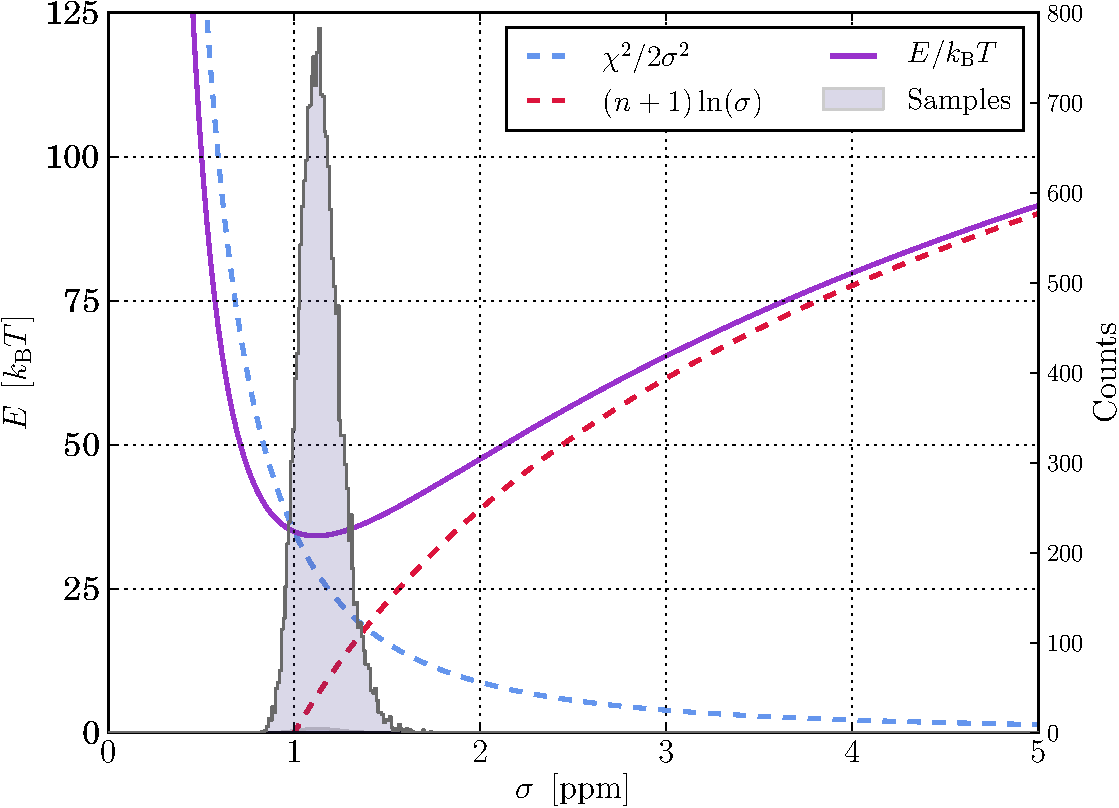
\includegraphics[width=0.45\textwidth]{figures/sigma_principle.pdf} }
    }
    \qquad
    \subfloat[Cauchy distribution]{
        {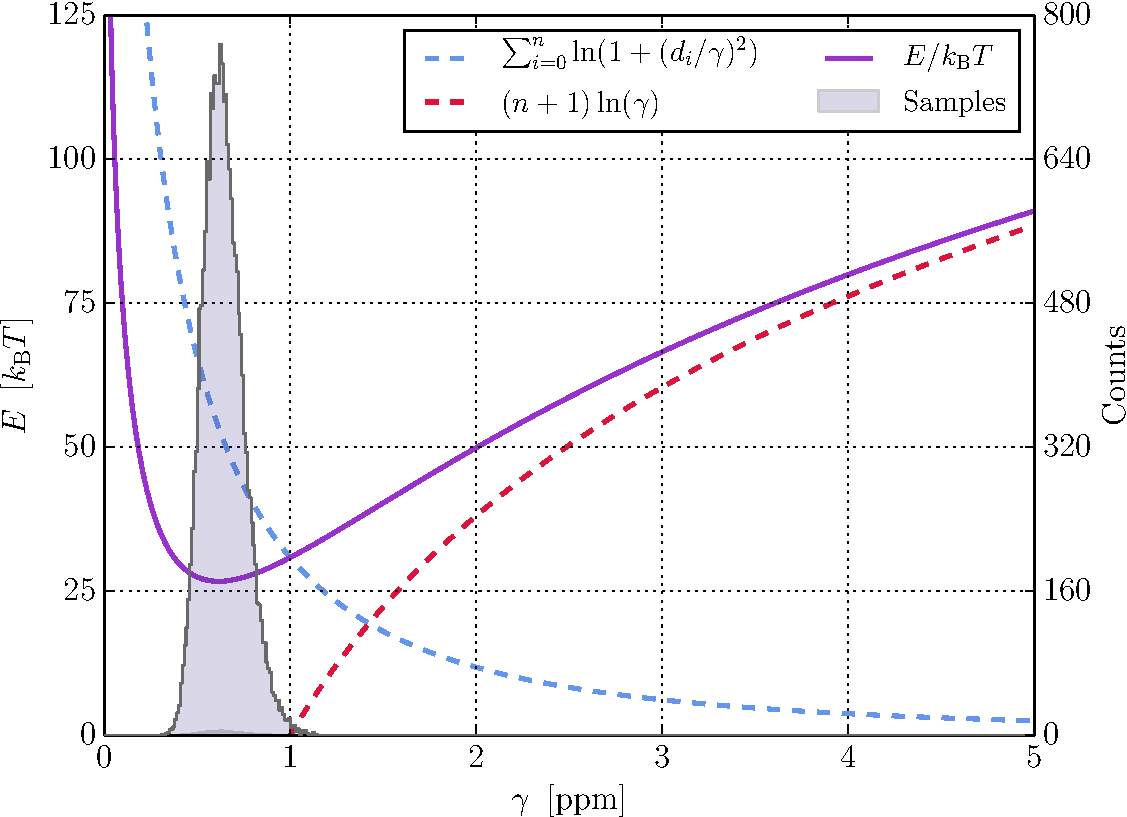
\includegraphics[width=0.45\textwidth]{figures/gamma_principle.pdf} }
    }
    \caption{Sampling of $\sigma$ and $\gamma$ for 2OED for Ca-chemical shifts. In this example $n = 55$ and $\chi^2 = 69.7$. Sampled values of the weight parameters clearly cluster around the minimum of the energy function.}
    \label{fig:example}%
\end{figure}

\subsection{Performance of energy functions}

Here folding simulation using 11 different variations of the energy function derived and mentioned previously are compared.
All energy functions have been implemented in the CamShift module in PHAISTOS, which was also used to run all simulations.
The test were carried out on Protein G and the engrailed homeodomain (ENHD). The reference structures were the structures 2OED and 1ENH.
An overview of the different simulation types can be found in Table~\ref{tab:prior_folds}.
For each energy function, 20 independent simulations were carried out for a total of 50,000,000 MC steps each.
Each simulation was initialized from a different random, extended strand.
Maximum likelihood estimated (MLE) values of the $\sigma$ and $\gamma$ weight parameters estimated take from the 7-protein test set reported in reference \cite{CamShift}.
For simulations where the weight parameter was sampled, an additional 500,000 Monte Carlo steps were carried out corresponding to the extra moves required to sample this weight (the computational overhead of these 500,000 moves is negligible).
Chemical shifts were calculated using the CamShift module.
All simulations used the PROFASI force field and sampling from either TorusDBN or TorusDBN-CS.
\begin{table}[h]
    \caption{Protocols used in the comparison of energy functions and success rates.}
    \begin{center}
    \begin{threeparttable}
    \begin{tabular}{l l l l l l}
                %& Force Field   &          & Correct fold\tnote{a} & Iterations/day\tnote{b}\\\hline
Energy type & Weight  & TorusDBN-mode & Sampling Bias & Correct sampling\tnote{a} & Correct scoring\tnote{b}\\\hline
Gauss         & Fixed/MLE   & Torus       & Biased   & 20/20  & 2/6  \\
Gauss         & Sampled & Torus       & Biased   &  0/0   & 0/0  \\
Cauchy        & Fixed/MLE   & Torus       & Biased   & 20/12  & 7/4  \\
Cauchy        & Sampled & Torus       & Biased   & 20/5   & 6/1  \\
Cauchy        & Sampled & Torus-CS    & Biased   & 20/20  & 4/2  \\
Cauchy        & Sampled & Torus       & No bias  &  0/0   & 0/0  \\
Cauchy        & Sampled & Torus-CS    & No bias  &  0/0   & 0/0  \\
Square-well   & Fixed   & Torus       & Biased   &  1/2   & 1/0  \\
Marginalized  & N/A     & Torus       & Biased   &  7/17  & 1/8  \\
No CS         & N/A     & Torus       & Biased   &  0/0   & 0/0  \\
No CS         & N/A     & Torus-CS    & Biased   &  8/10  & 2/0
    \end{tabular}
    \begin{tablenotes}
        \item[a] Number of threads with a CA-RMSD of $<5$ \AA\ (using all residues). Listed as xx for Protein G and yy for ENHD, i.e.~xx/yy.\\
        \item[b] Number of threads where the lowest energy sample has a CA-RMSD of $<3$ \AA\ (using all residues). Listed as xx for Protein G and yy for ENHD, i.e.~xx/yy.\\
    \end{tablenotes}
    \end{threeparttable}
    \end{center}
    \label{tab:prior_folds}
\end{table}

In two simulations, the bias was removed from the simulation, which corresponds to an unbiased simulation.
Two reference simulations were carried out with no chemical shift energy-function, in order to analyze the effect of sampling from TorusDBN and the effect of the PROFASI force field.
The simulations used a mix of 40\% biased CRISP-moves, 10\% biased pivot moves and 50\% uniform side chain moves.
The simulation was carried out in the multicanonical ensemble via MUNINN.
Minimum and maximum $\beta$-values were set to 0.3 and 1.05, and the temperature was set to 300K.
In all simulations, the number of threads which had samples below thresholds of 5, 3, 2 and 1 \AA~CA-RMSD from the crystal structure was recorded.
Similarly, the number of threads in which the lowest energy structure was below thresholds of 5, 3, 2 and 1 \AA~CA-RMSD from the crystal structure was recorded.
These figures are used to analyze whether sampling or correct energy scoring is are limiting factors in the particular simulations.
The energy was calculated as the PROFASI energy multiplied by $k_{\mathrm{B}}T$ plus the chemical shift energy term plus the log-likelihood calculated from TorusDBN.
An overview of these results can be seen in Fig.~\ref{fig:cauchy_results} (only simulations that had any samples below 5 \AA~CA-RMSD from the crystal structure are shown).

For both proteins, using a Gaussian model and sampling the $\sigma$ uncertainty does not lead to meaningful values for $\sigma$.
In short, PHAISTOS is able to generate a structure which has no difference between experimental and calculated chemical shifts for a certain atom type.
Consequently, the value of $\sigma$ converges to zero, which effectively freezes the structure in the simulation.
The simulations in which the move-bias from TorusDBN and TorusDBN-CS was removed did not sample any structures below 

For simulations using Gaussian or Cauchy types of energy function all thread had samples below 5 \AA~CA-RMSD from the crystal structure for Protein G and between 5-20 for ENHD 
In the simulation using the square-well potential only 1 thread had samples below 5 \AA~for Protein G  and only 2 for ENHD.
For the simulation with marginalized weight parameters, the same figures were 7 and 17, respectively.
The reference simulations with no chemical shift in the energy function had no samples below 5 \AA~for biased sampling from TorusDBN, but 8 and 10 threads below 5 \AA~for biased sampling from TorusDBN-CS.

Comparing the number of threads for which the lowest energy sample was below 3 \AA~CA-RMSD from the crystal structure.
For both proteins, using fixed weights is somewhat better than using sampled weights with the Cauchy distribution.
The result for the square-well potential cannot be interpreted to a statistical significance because only one and two threads were close to the correct fold, but one thread correctly identified the folded state below 3 \AA~CA-RMSD as the lowest energy for Protein G.

In conclusion, the Gauss and Cauchy error models perform well in sampling and scoring.
The fixed MLE weights seem to be work equally well to sampling weights for the cauchy distribution, with no substantial differences.
The performance of the energy with marginalized weights generally performed worse in guiding the sampling, but well in scoring samples for ENHD.
The square-well potential did not improve the sampling much.
The reason why it has previously been shown to work well, might be that it was combined with a better force-field (AMBER03) to which it was specifically designed.
One clear conclusion is that it is useful to not remove the bias from TorusDBN, and keeping the TorusDBN-CS bias seems guide folding significantly more. Even though this formally constitutes is double-counting of effect of knowledge about chemical shifts, this practice seemingly has no adverse effects.




\begin{figure}%
    \centering
    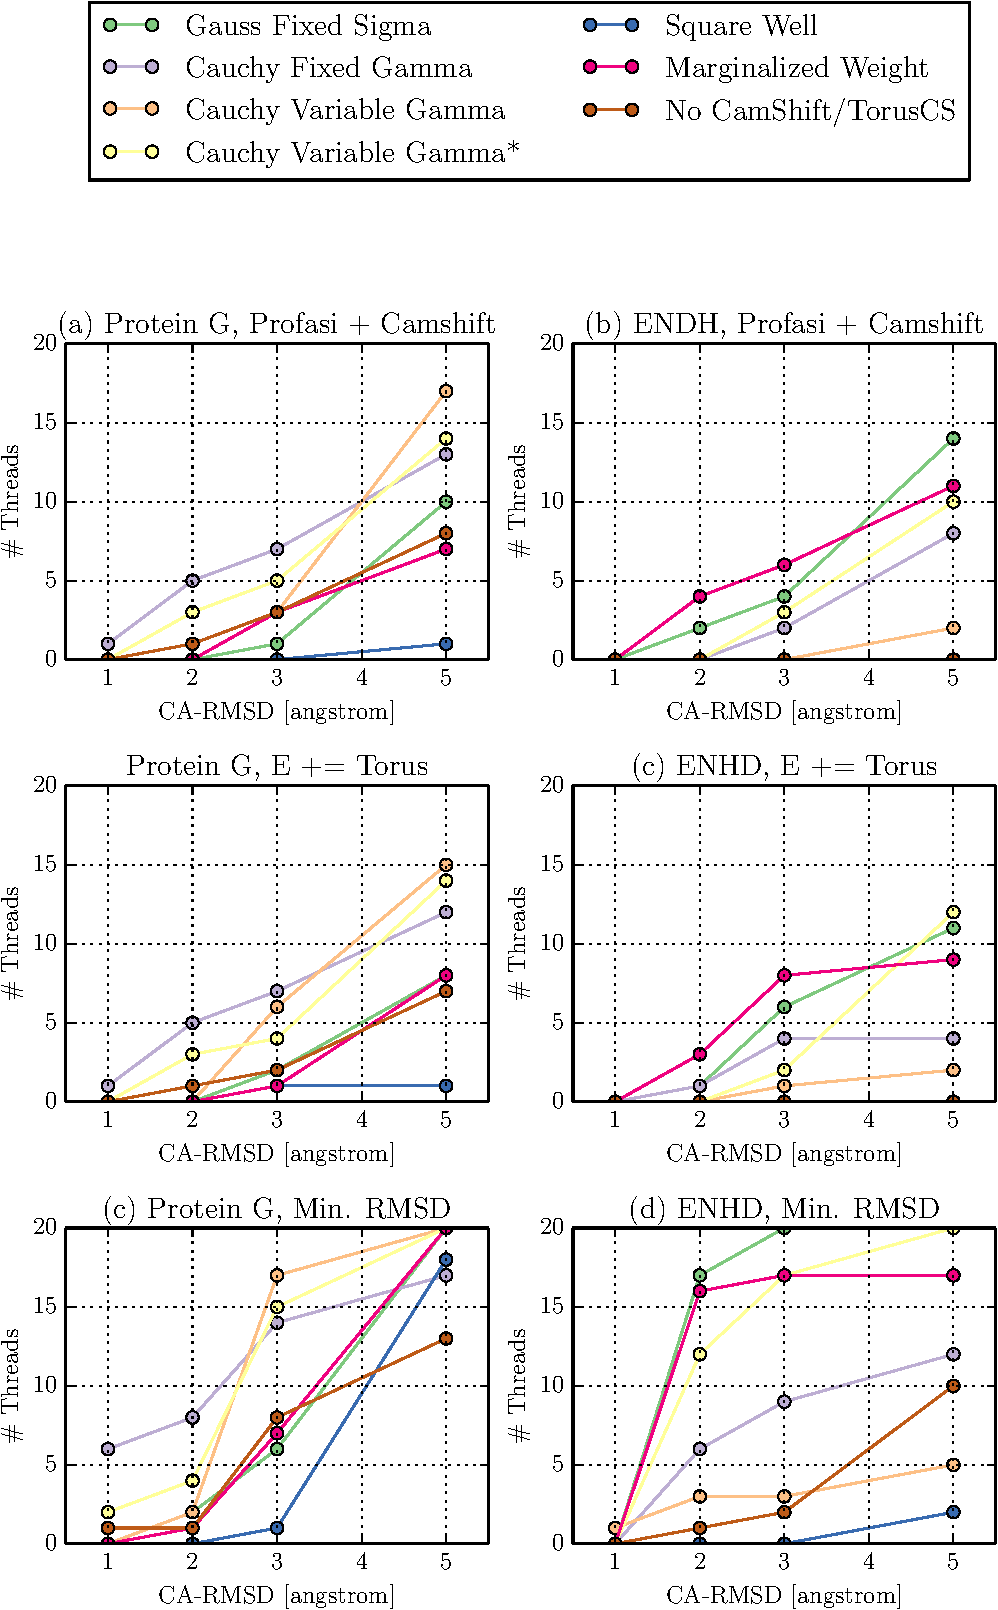
\includegraphics[width=0.75\textwidth]{figures/cauchy_folds/cauchy_folds.pdf}
    \caption{Overview of folding simulations using 7 different chemical shift energy types. Sampling was biased by TorusDBN and the PROFASI energy term was used as well.
             In (a) and (b) the number of threads where the lowest energy samples are under thresholds of 1, 2, 3 and 5 \AA~CA-RMSD from the crystal structure is plotted. 
             The energy here is calculated as the PROFASI energy multiplied by $k_{\mathrm{B}}T$ plus the chemical shift energy term. 
In (c) and (d), the log-likelihood from TorusDBN has been added to the total energy.
In (e) and (f), the number of threads in which samples are found below under thresholds of 1, 2, 3 and 5 \AA~CA-RMSD from the crystal structure is plotted. 
*In this simulation TorusDBN-CS is used instead of TorusDBN.}
    \label{fig:cauchy_results}%
\end{figure}



% \subsection{Generative probabilistic models}
% 
% Another way to introduce the prior distribution for a protein structure is to bias the conformational sampling. 
% Conventional conformational sampling will proposed $(\phi, \psi)$ backbone angles uniformly (i.e. in the range $[-180^{\circ}, 180^{\circ}]$ and let the energy function filter and construct the target distribution (e.g. the canonical ensemble, etc.) via energy evaluation.
% Since only a fraction of the possible $(\phi, \psi)$ backbone angles are allowed (i.e. the Ramachandran plot), it is computationally very convenient to only sample from the allowed regions.
% Using biased sampling, energy evaluation of structures that are obviously in sterically unfavored regions is eliminated with high efficiency.
% 
% Taking the biased sampling one step further, it is possible to have the biased sampling via TorusDBN conditioned on a set of chemical shifts.
% This sampling is carried out via the TorusDBN-CS model by Boomsma \textit{et al.} TorusDBN-CS is trained on all chemical shift data available in the RefDB database, that is 1349 protein structures with their corresponding chemical shifts. This includes both experimental X-ray crystal and NMR structures.
% 
% In most cases TorusDBN-CS model is able to restrict the conformational sampling of $(\phi, \psi)$ angles to not only the Ramachandran plot, but also the correct region (e.g. alpha-helix, beta-sheet), etc.
% However, since the data set is smaller than that of the TorusDBN (non-CS) model TorusDBN-CS will occasionally be less restrictive than TorusDBN and may sample outside the Ramachandran plot.
% 
% 
% 
% \subsubsection{TorusDBN and TorusDBN-CS}
% 
% 
% \subsubsection{BASILISK}
% 
% Similarly to biased sampling in TorusDBN, it is possible to sample side-chain angles via BASILISK. There is currently no chemical shift dependent equivalent to BASILISK, but such a module is currently in our plans.
% 
% 
% \begin{figure}
%     \centering
%     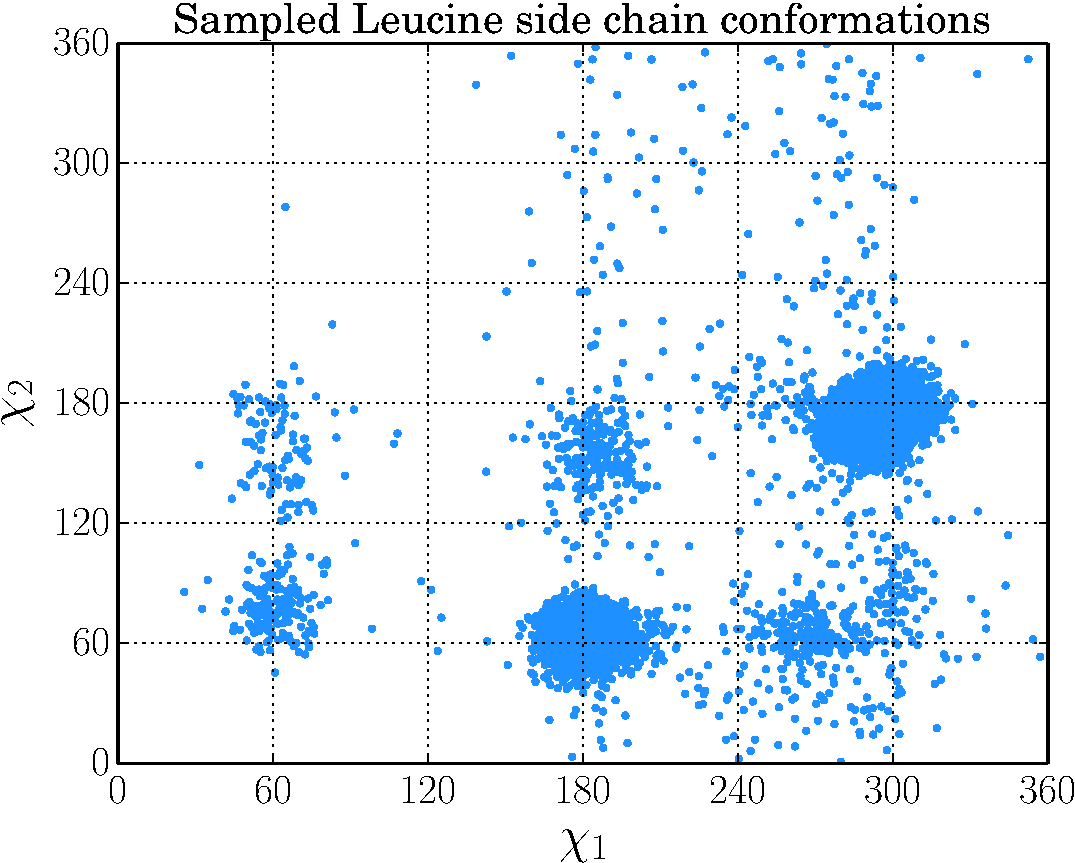
\includegraphics[width=0.65\textwidth]{figures/leu_sc.pdf}
%     \caption{Example of Leucine rotamer conformations sampled from BASILISK. Values were sampled using the backbone conformation dependent option via the FragBuilder Python API.}
%     \label{fig:leu_sc}
% \end{figure}

% \chapter{Graphical User Interface for PHAISTOS}
% 
% Setting up simulations in PHAISTOS requires expert knowledge about the program. 
% Firstly, while all modules and settings have reasonable default settings, there are still many things that cannot be specified via default alone, and secondly, the complete list of settings in PHAISTOS is around 2500 options that must be set or taken as default values.
% 
% In order to make PHAISTOS more available to new users, I wrote a GUI can set up most simulations for most of the simulations covered by this thesis.
% The GUI for PHAISTOS is aptly named Guistos and is written in Python 2.x using TkInter.
% 
% Using the GUI the user is only presented with the three most basic choices for setting up the simulation.
% These are (1) choice of energy terms, (2) type of Monte Carlo simulation and finally (3) a selection of Monte Carlo moves.
% Setting up these via Guistos is discussed next.
% 
% \begin{figure}
%     \centering
%     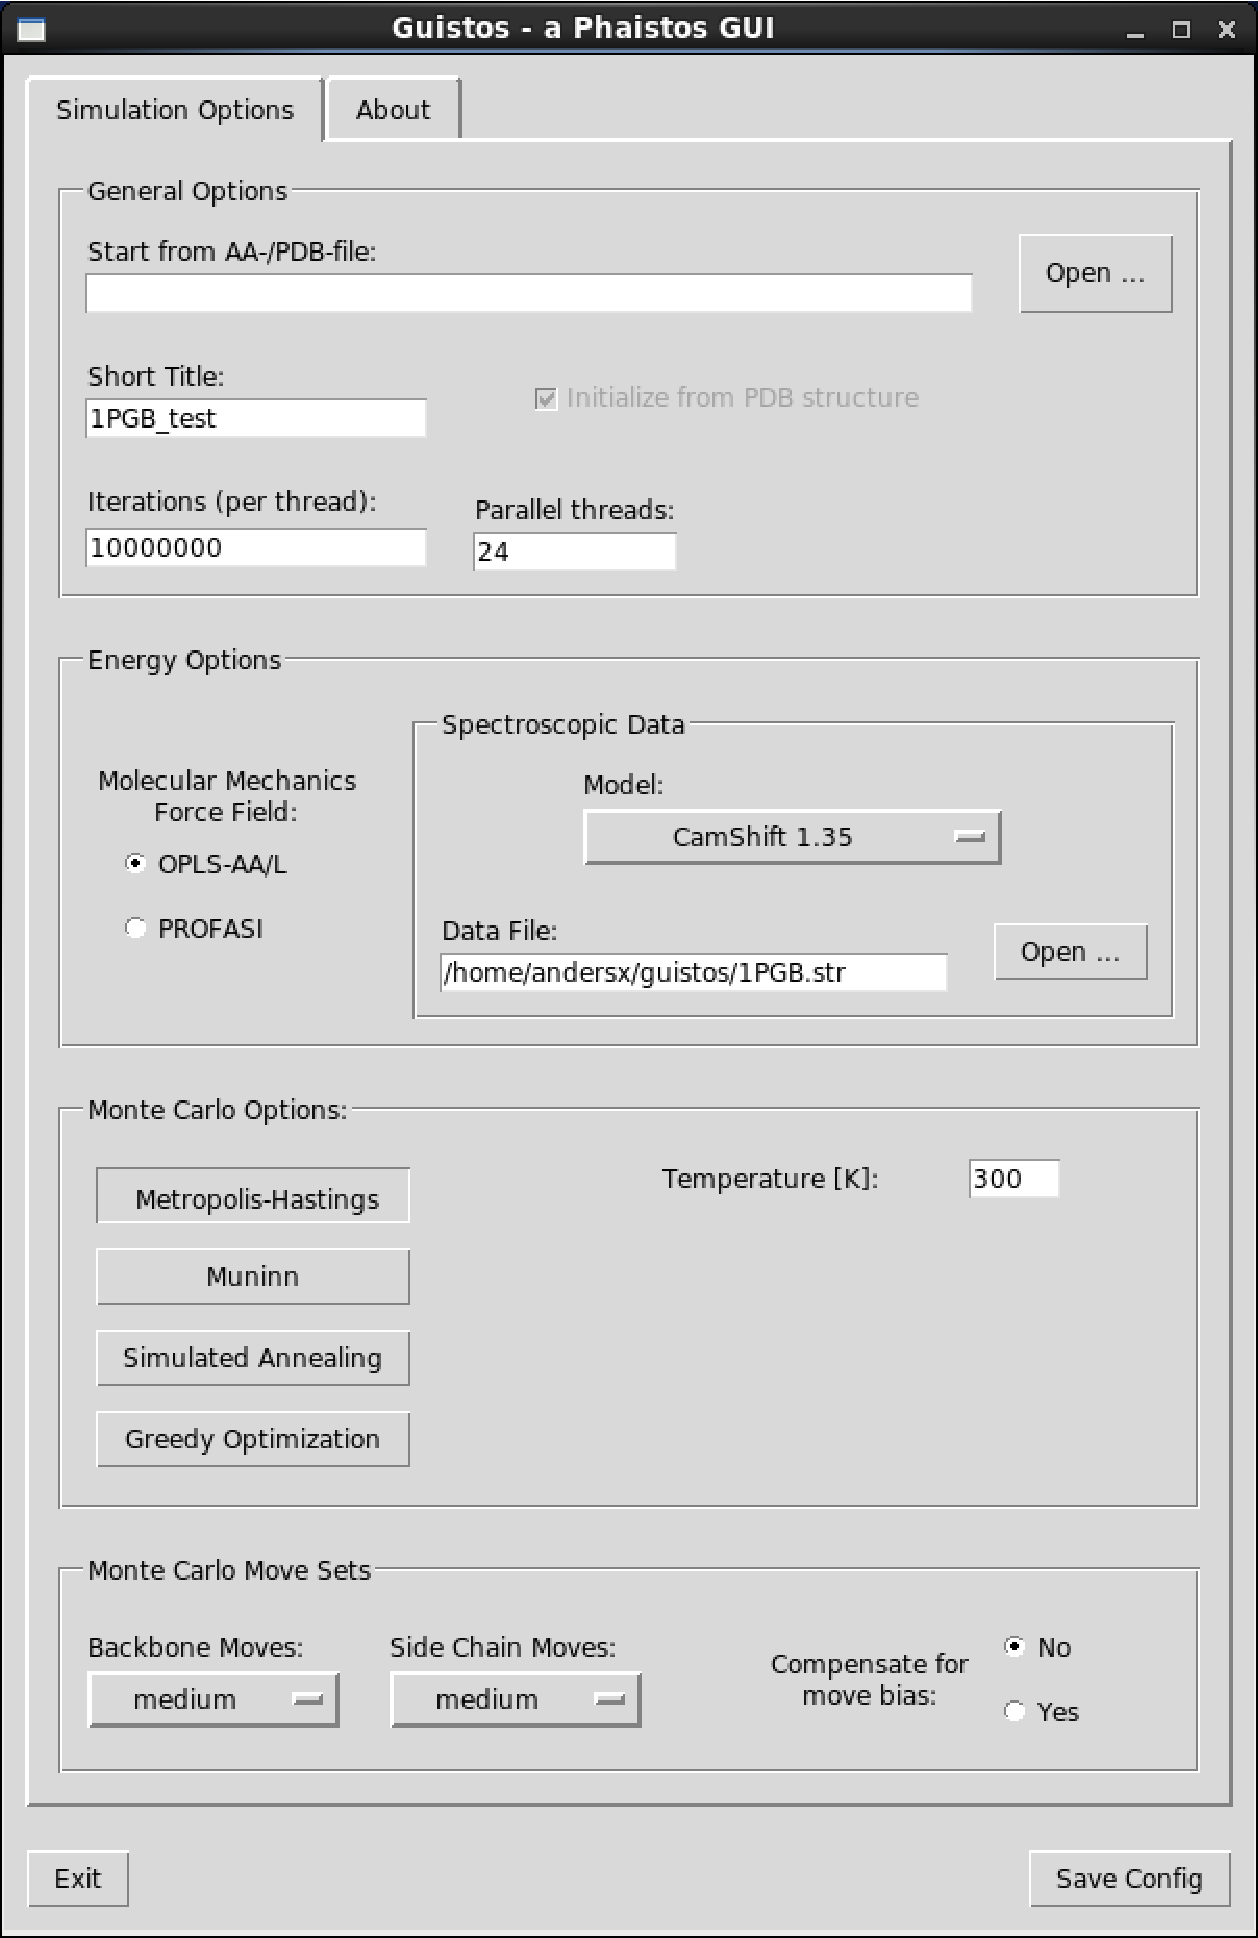
\includegraphics[width=0.70\textwidth]{figures/guistos.pdf}
%     \caption{Screenshot of Guistos}
%     \label{fig:guistos}
% \end{figure}
% 
% \subsubsection{Energy Options}
% 
% Firstly, the Energy Options section allows the user to select the molecular mechanics force field.
% Currently two force fields are supported in PHAISTOS, which are the OPLS-AA/L force field with a GB/SA solvent model, and the PROFASI coarse grained force field.
% Use of the PROFASI force field requires the Monte Carlo moves to restraint the bond angle and lengths in the protein to Engh-Huber standard values.
% This is automatically done if the PROFASI force field is selected. 
% Conversely, the OPLS-AA/L force field includes energy terms for bond angles and lengths and these are degrees of freedom in the simulation if the OPLS-AA/L force field is selected.
% 
% Additionally, the Energy Options section allows the user to add restrains from one type spectroscopic data.
% Currently energy terms based on CamShift 1.35 and ProCS are supported.
% These options requires a NMR-STAR formatted file containing experimental chemical shifts.
% 
% 
% \subsubsection{Monte Carlo Options}
% 
% This section allows the user to select the four types of Monte Carlo simulation offered by PHAISTOS and the only the most basic options to set up that particular simulation:
% Metropolis-Hastings offers the choice of a constant temperature (in Kelvin).
% Muninn and Simulated Annealing offer the choice of a temperature range (in Kelvin), and additionally Muninn offers the choice between multicanonical or $1/k$ sampling.
% Greedy Optimization does not offer any customizable option. 
% 
% \subsubsection{Monte Carlo Move Sets}
% 
% Selecting a good mix of the different Monte Carlo moves offered by PHAISTOS can significantly speed up convergence of a simulation, compared to using an inferior move set.
% Choosing a good set of moves is in the opinion of this author currently somewhere in between black art and sheer luck, and requires a good deal of experience with simulations in PHAISTOS.
% 
% To make it easier for new users, three move sets have been predefined using the experience of this author.
% These are named "small", "medium" and "large".
% The "small" move set is intended for uses such as refinement or sampling around a compact native state, 
% while the "medium" move set is intended for folding simulations that start from extended, but are expected to also sample a native state, 
% and finally the "large" move set is intended for sampling conformational space quickly, but will have problems with sampling compact structures.
% All move sets sample from TorusDBN (backbone angles) and BASILISK (side chain angles), and an option to remove this bias is also present.
% 
% \subsubsection{Using Guistos}
% 
% Guistos is freely released under the open source two-clause BSD-license, and can be downloaded from \url{https://github.com/andersx/guistos}. A screenshot of Guistos can be seen in Fig.~\ref{fig:guistos}. 
% After specifying all relevant settings in the Guistos window, a configuration-file is saved by pressing the "Save Config" button.
% A simulation in PHAISTOS can the be executed via the following command:
% \begin{lstlisting}
% ./phaistos --config-file my_simulation.config
% \end{lstlisting}








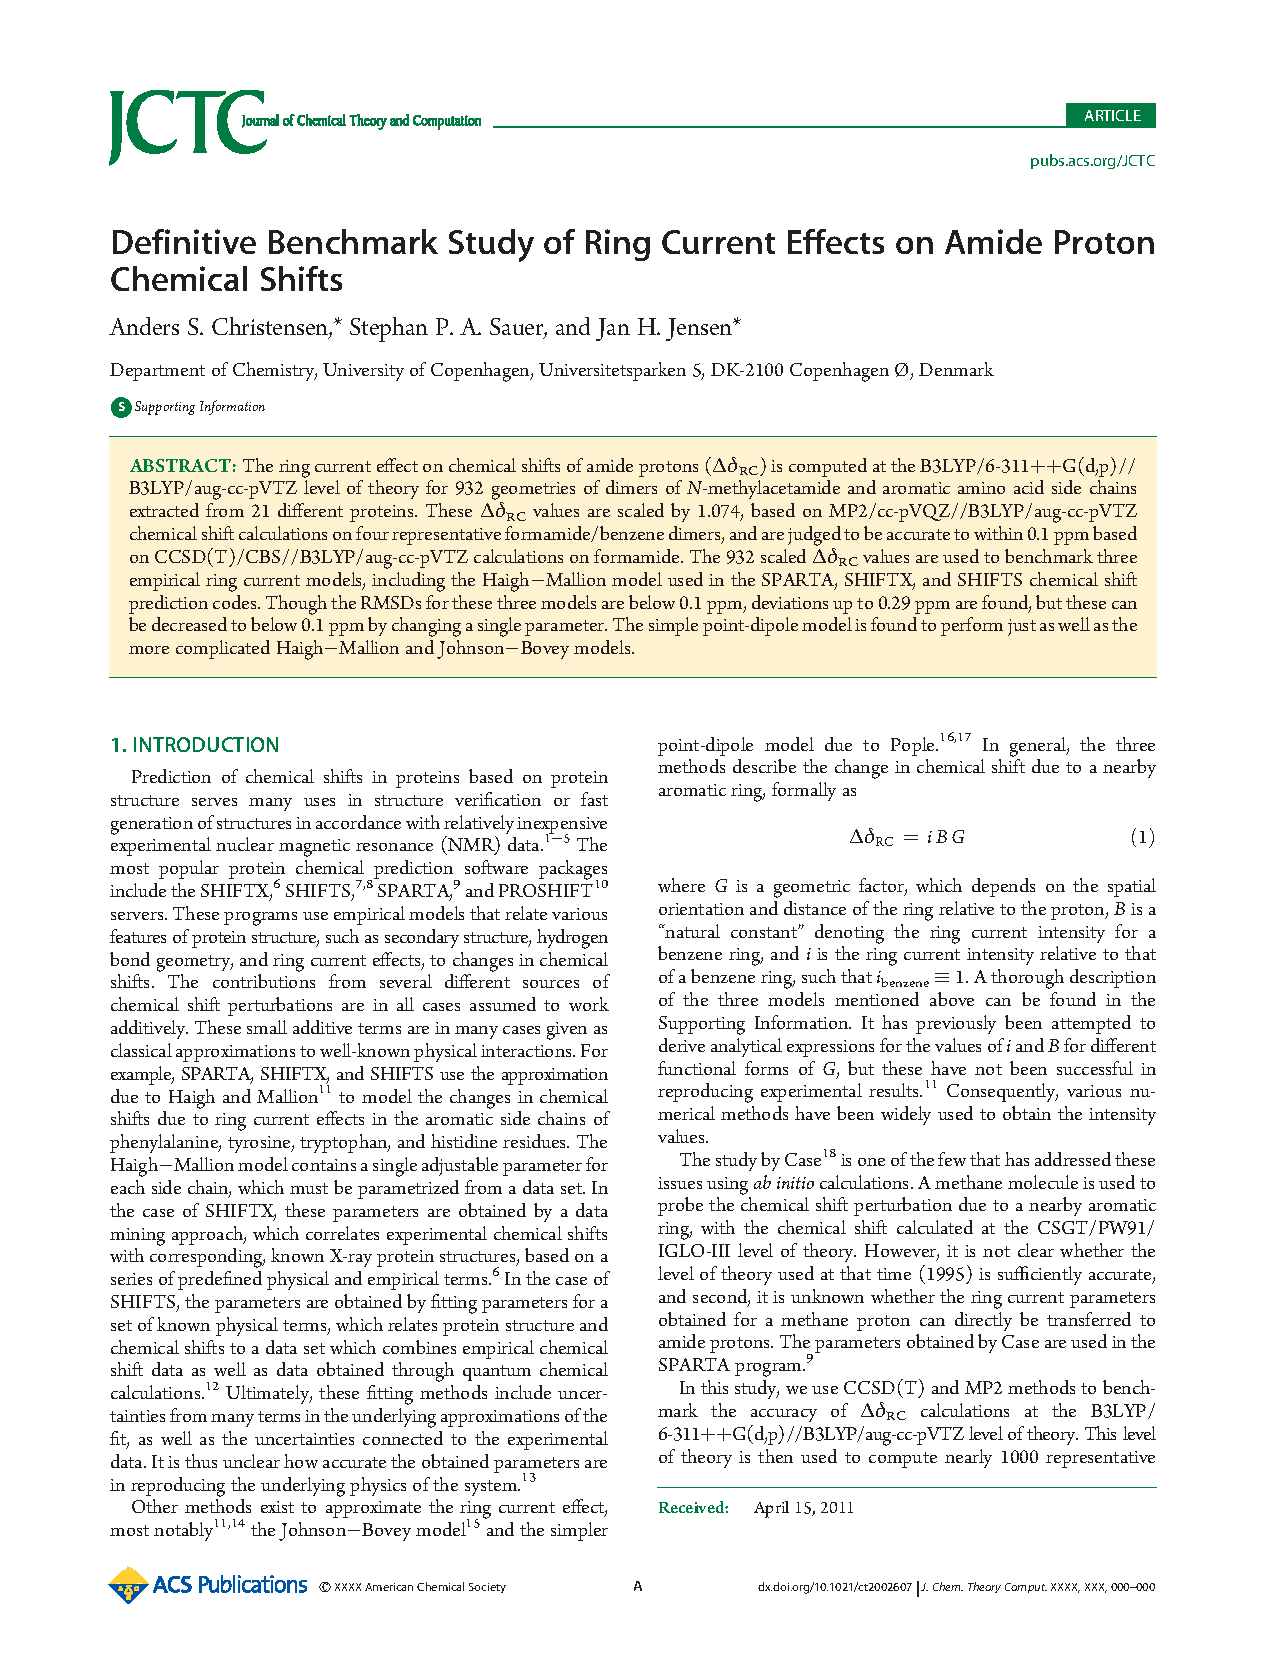
\includepdf[pages={1-7}]{papers/ChristensenJCTC2011.pdf}
\bibliography{tex/references}
\end{document}
